\subsection{Estilos arquitectónicos}

Para dar solución a los requerimientos, Kwii Platform adopta un estilo arquitectonico basado en microservicios, teniendo como componentes encargados de la presentación de nuestros servicios y el manejo de los usuarios, los clientes movil y web, además de una familia de microservicios construida especificamente para el manejo de la lógica de Kwii Platform, la conexion de estos familia microservicios es posible a traves del uso del conector REST.

\subsubsection{Uso del estilo de microservicios}

Consecuentemente, Kwii Platform aplica un Patron de microservicios estructurado de la siguiente manera:\\ 

5 componentes que encapsulan funcionalidades concretas de la aplicación (administracion de usuarios, sesion, salas de chat, mensajes y un componente de notificación), adicionalmente se tiene un componente adicional encargado de sincronizar los demas ademas de exponer la funcionalidad completa de la aplicación a los clientes.

\begin{center}
    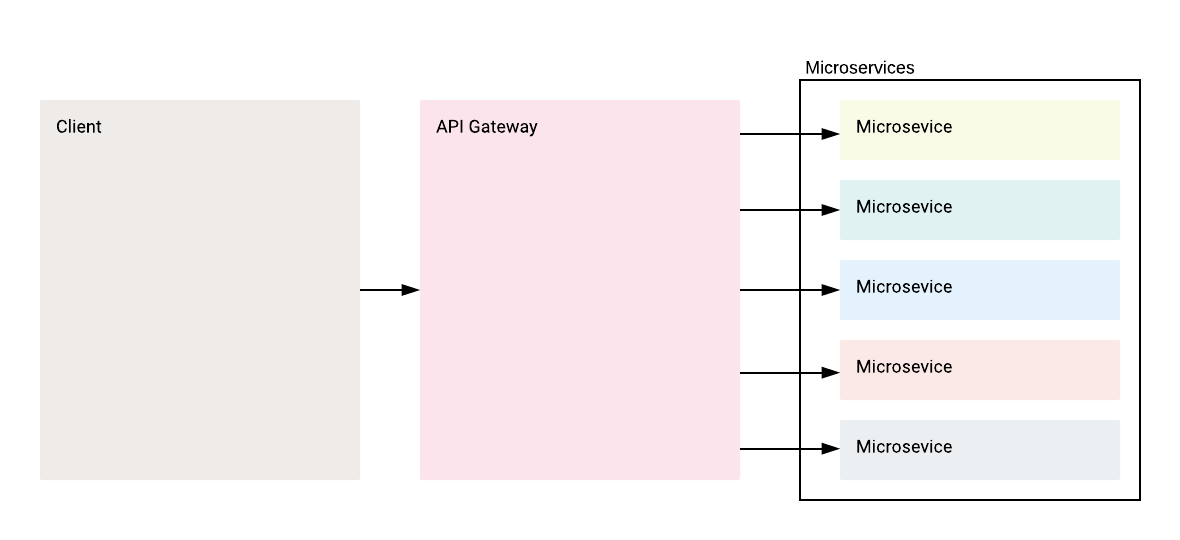
\includegraphics[width=14cm]{Figures/P2/microservices.png}    
\end{center}


\subsubsection{Uso del estilo REST}

REST se ha consolidado como el estilo más adecuado cuando el protocolo de comunicacion es HTTP para obtener datos y aún más si la representación de estos datos es en XML o JSON, siendo esta última la representación elegida para las entidades de esta aplicación.



\subsection{Patrones arquitectónicos}

Cada uno de los microservicios a su vez utiliza un patron arquitectonico para poder cumplir con su funcion especifica, el patron usado por cada uno de ellos se describe a continuación: \\

\subsubsection{MVC (Modelo Vista Controlador)}

Este modelo se utiliza en cuatro de los cinco microservicios (usuarios, autenticación y notificaciones y chat-room), estos servicios manejarán las entidades a través de controladores, los cuales podrán renderizar respuestas a peticiones HTTP en formato JSON, estas representaciones actuarán como vistas.


\subsubsection{MTV (Model Template View)}

En el caso del microservicio de chat este modelo no solo resulta ser el más adecuado para el framework en el que se desarrolla (Django), sino que accede a la base de datos a través del modelo, y en lugar de utilizar una vista para la capa de presentación, utiliza una plantilla. que permite determinar con mayor facilidad que cosas se muestran en las vistas, que en este caso hacen el rol de describir la lógica del negocio. Esto último resulta ser útil para el motor de bases de datos noSql que se usa en este caso (MongoDB).



    